\documentclass[tikz,border=10pt]{standalone}
\usetikzlibrary {scopes}
\usetikzlibrary{arrows.meta}
\begin{document}

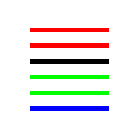
\begin{tikzpicture}[ultra thick]
	\begin{scope}[red]
		\draw (0mm,10mm) -- (10mm,10mm);
		\draw (0mm,8mm) -- (10mm,8mm);
	\end{scope}
	\draw (0mm,6mm) -- (10mm,6mm);
	\begin{scope}[green]
		\draw (0mm,4mm) -- (10mm,4mm);
		\draw (0mm,2mm) -- (10mm,2mm);
		\draw[blue] (0mm,0mm) -- (10mm,0mm);
	\end{scope}
\end{tikzpicture}


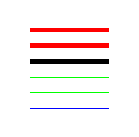
\begin{tikzpicture}
	{ [ultra thick]
			{ [red]
				\draw (0mm,10mm) -- (10mm,10mm);
				\draw (0mm,8mm) -- (10mm,8mm);
			}
		\draw (0mm,6mm) -- (10mm,6mm);
	}
	{ [green]
		\draw (0mm,4mm) -- (10mm,4mm);
		\draw (0mm,2mm) -- (10mm,2mm);
		\draw[blue] (0mm,0mm) -- (10mm,0mm);
	}
\end{tikzpicture}

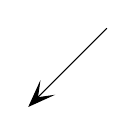
\begin{tikzpicture}
	{   [arrows = {-Stealth[length=10pt, inset=5pt]}]
	\draw (-5,-5)-- ++(-1,-1);
	}
\end{tikzpicture}

\end{document}
